\documentclass[lettersize,journal]{IEEEtran}
%\documentclass[conference]{IEEEtran}
\usepackage{amsmath,amsfonts}
\usepackage{algorithmicx}
\usepackage{algorithm}
\usepackage{array}
\usepackage[caption,font=normalsize,labelfont=sf,textfont=sf]{subfig}
\usepackage{textcomp}
\usepackage{stfloats}
\usepackage{url}
\usepackage{verbatim}
\usepackage{graphicx}
\usepackage{cite}
\usepackage{tabularx}
\usepackage{scalefnt}
%\documentclass[a4paper, 10pt, conference]{ieeeconf}   
%\usepackage{blindtext, graphicx}
%\usepackage{listings}
%\lstset { %
%	language=C++,
%	numbers=left,
%	breaklines=true,
%	xleftmargin=4em,
%	resetmargins=true,
%	basicstyle=\footnotesize,
%	numberstyle=\footnotesize,
%}
%\usepackage{graphicx}
%\usepackage{amsmath}
%\usepackage{tabularx}
\usepackage[font=normalsize]{caption}

%Pacote para acentos [Por TIAGO]
\usepackage[portuguese]{babel}
%\addto\captionsportuguese{
%	\renewcommand{\figurename}{Figura}
%	\renewcommand{\tablename}{Tabela}
%}
% updated with editorial comments 8/9/2021
\hyphenation{op-tical net-works semi-conduc-tor IEEE-Xplore}

\begin{document}

\title{Confiabilidade de Linhas de Transmissão\\ Utilizando Sistema Sul Brasileiro \\ com 32 Barras}

\author{Leonardo Felipe da Silva dos Santos,~\\ \IEEEmembership{Centro de Excelência em Energia e Sistemas de Potência (CEESP),\\ Programa de Pós-Graduação em Engenharia Elétrica,~\\ Universidade Federal de Santa Maria \\ Santa Maria, Brasil \\ leonardo.santos@acad.ufsm.br}}
        % <-this % stops a space
% \thanks{This paper was produced by the IEEE Publication Technology Group. They are in Piscataway, NJ.}% <-this % stops a space
% \thanks{Manuscript received April 19, 2021; revised August 16, 2021.}}

% The paper headers
% \markboth{Journal of \LaTeX\ Class Files,~Vol.~14, No.~8, August~2021}%
% {Shell \MakeLowercase{\textit{et al.}}: A Sample Article Using IEEEtran.cls for IEEE Journals}

% \IEEEpubid{0000--0000/00\$00.00~\copyright~2021 IEEE}
% Remember, if you use this you must call \IEEEpubidadjcol in the second
% column for its text to clear the IEEEpubid mark.

\maketitle

\begin{abstract}
This document describes the most common article elements and how to use the IEEEtran class with \LaTeX \ to produce files that are suitable for submission to the IEEE.  IEEEtran can produce conference, journal, and technical note (correspondence) papers with a suitable choice of class options. 
\end{abstract}

\begin{IEEEkeywords}
Article submission, IEEE, IEEEtran, journal, \LaTeX, paper, template, typesetting.
\end{IEEEkeywords}

\section{Introdução}
\IEEEPARstart{O}{} sistema elétrico brasileiro é constituído fundamentalmente por usinas hidrelétricas de grande porte, quais essas criam desafios para linhas de transmissão (LTs), quais hoje no Brasil o sistema em anel propõem uma segurança para o escoamento de energia e também cria um sistema de troca de energia entre as regiões, assim o sistema pode encontrar problema para distribuição de diversas cargas localizadas em locais pontuais com falta de geração ou demandas quais superam a intercambialidade de regiões.

Assim as capacidades da transmissão de energia ficam voltadas a confiabilidade do sistema elétrico de potência para escoamento dos geradores, quais o Brasil é referencia em usar hidrelétricas em sua grande maioria, normalmente localizadas na parte norte do Brasil por apresentar uma hidrologia mais favoráveis a geração hidrelétrica.

Este artigo visando a utilização do sistema de transmissão sul brasileiro de 32 barras (STSB-32) para criar o cenário de primeira ordem do diagrama de cortes e o cenário de segunda ordem, assim numerados utilizando os métodos de enumeração de estados do critério N-1 e N-2\cite{Lazari}.

Este artigo tem como proposta analisar o comportamento do Sistema STSB-32 conforme as pontos de operação propostos, assim como utilizar os modelos de confiabilidade compostos para calcular a confiabilidade do sistema n-2, se utiliza o \textit{software} ANAREDE, para todos os objetivos deste artigo, pois o ANAREDE é utilizado para o planejamento seguro do Sistema Interligado Nacional – SIN.

Este artigo está organizado da seguinte maneira. A seção 2 aborda a confiabiliade de sistemas elétricos de potência, com uma revisão do assunto. A seção 3 explana modelagem do sistema e as simulações realizadas para os dois cenários abordados. Os resultados são discutidos na seção 4. Finalmente na seção 5 apresentado as conclusões e as contribuições do estudo.

\section{Confiabilidade de Sistemas \\ Elétricos de Potência}

Qualquer sistema de potência está sujeito a falhas pontuais, tanto em equipamentos dispostos nas subestações quanto em linhas de transmissão, quais estas falhas podem comprometer a operação em parte ou todo sistema de potência, qual pode inviabilizar o fornecimento de energia em vários pontos e até mesmo para consumidores finais.

Assim a confiabilidade por meio da análise dos índices probabilísticos do sistema, combinado com julgamentos sobre critérios pré-estabelecidos e com um julgamento próprio. Porém hoje a confiabilidade utiliza métricas erradas sobre as linhas de transmissão, qual os valores são definidos por um geral e não por linha, quais esses históricos são recentes, assim não tendo dados de todos os pontos, afinal os sistema elétrico de potência é relativamente novo no Brasil.

Toda a parte de confiabilidade é baseada em grandes técnicas de análise, que utiliza princípios e conceitos da matemática fornecidos pela teoria de probabilidade\cite{Armando2022}. A análise de confiabilidade busca, basicamente, analisar o risco de não atendimento à demanda do sistema de potência.

Com a utilização destes conhecimentos pode-se calcular quais as chances de que um determinado sistema ou componente possa falhar, assim criando modelos de confiabilidade quais podem ser mensuradas conforme modelos pré-estabelecidos ou normas vigentes como no caso das regras dos serviços de transmissão de energia elétrica no Sistema Elétrico Nacional regulamentado pela Agência Nacional de Energia Elétrica - ANEEL.

\begin{figure}[h]
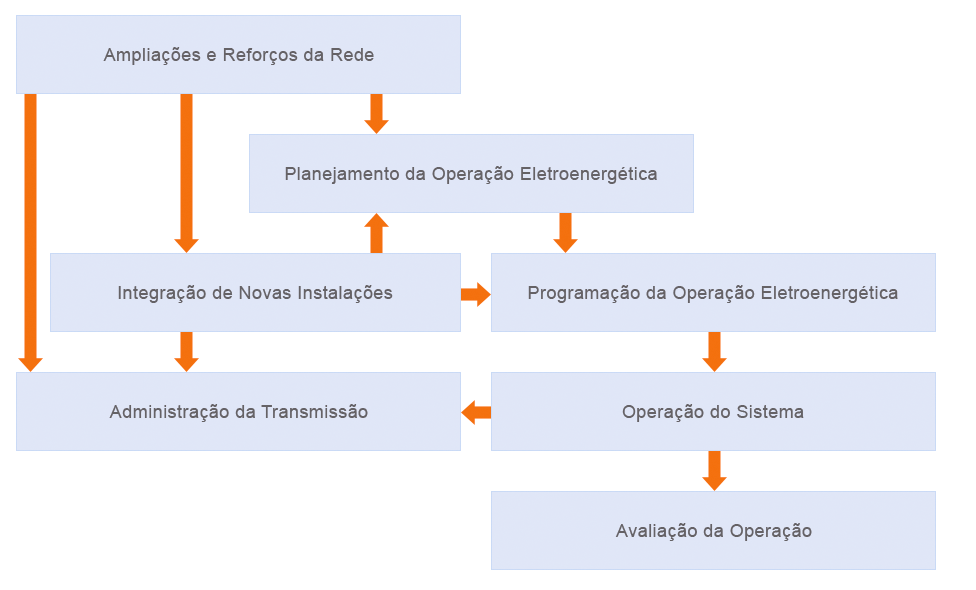
\includegraphics[width=0.5\textwidth]{Figuras/ONS_ABRANGENCIA.png}
\centering
\caption{Área de Atuação da ONS perante o Sistema.}
\label{figura: ONS_AREA}
\end{figure}

\newpage

Já quem faz a operação do sistema nacional é o operador naciona do sistema elétrico (ONS), qual faz desde o planejamento elétrico até operação do sistema como um todo, como mostrada na Figura \ref{figura: ONS_AREA}, a abrangência da ONS perante o SIN.

\subitem{Níveis Hierárquicos}

A análise de confiabilidade pode abranger três níveis
hierárquicos, conforme apresentado na Figura \ref{figura: Niveis_Hierarquicos} \cite{Cassula2003}:
\begin{enumerate}
	\item Nível Hierárquico 0 (NH0): Abrange o estudo de confiabilidade ligado ao sistema energético isolado aos demais, normalmente se analisa a confiabilidade de projeto e funcionamento;
	\item Nível Hierárquico 1 (NH1): Abrange o estudo de confiabilidade ligado a geração de energia;
	\item Nível Hierárquico 2 (NH2): Abrange o estudo de confiabilidade ligados a transmissão e geração de energia;
	\item Nível Hierárquico 3 (NH3): Abrange o estudo de confiabilidade ligados a distribuição, transmissão e geração de energia.
\end{enumerate}

\begin{figure}[h]
	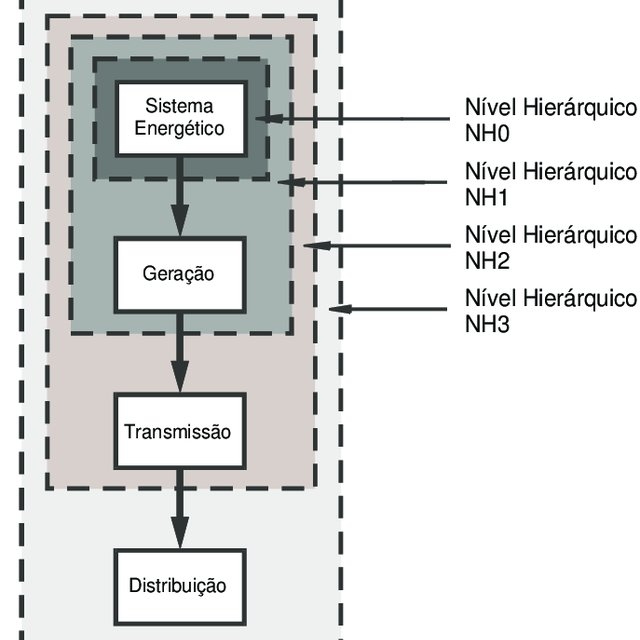
\includegraphics[width=0.3\textwidth]{Figuras/Figura-1-Niveis-Hierarquicos-de-um-Sistema-de-Potencia.jpg}
	\centering
	\caption{Níveis Hierárquicos de um Sistema de Potencia\cite{Cassula2003}.}
	\label{figura: Niveis_Hierarquicos}
\end{figure}

Atualmente devido a dimensão dos problemas trabalhamos apenas com o NH2, assim montando o problema em razão das falhas em linhas de transmissão quais já foram modeladas e levantadas.

\section{Modelagem e Simulações}

Nesta seção apresentam-se as caracteristicas do sistema de transmissão sul brasileiro com 32 barras simulado no \textit{software} \textbf{ANAREDE}, para o cenário proposto para níveis de carregamento e níveis de geração, como um ponto de operação qual haveria contingências se houvesse alguma violação de tensão ou fluxo de potência, assim como considerar contingências os casos divergentes a partir do ponto de operação descrito na Tabela \ref{tabela: Nivel_Carregamento}.

\newcolumntype{Y}{>{\centering\arraybackslash}X}
\begin{table}[ht]
	\caption{Configuração do Nível de Carregamento(MW)}
	\label{tabela: Nivel_Carregamento}
	\centering
	\begin{tabularx}{.4\textwidth}{| Y | Y | Y |}
		\hline
		\multicolumn{3}{|c|}{Nível de Carregamento (MW)} \\
		\hline
		Área 1 & Área 2 & Área 3 \\
		\hline
		3100 & 7800 & -4500 \\
		\hline
	\end{tabularx}
\end{table}

Assim como o nível de carregamento foi definido em cada área do sistema, o nível de geração também foi previamente definido conforme a Tabela \ref{tabela: Nivel_Geracao}.

\begin{table}[ht]
	\caption{Configuração do Nível de Carregamento(MW)}
	\label{tabela: Nivel_Geracao}
	\centering
	\begin{tabularx}{.4\textwidth}{| Y | Y |}
		\hline
		\multicolumn{2}{|c|}{Nível de Geração } \\
		\hline
		Área 1 & Área 2 \\
		\hline
		-20\% & -20\% \\
		\hline
	\end{tabularx}
\end{table}

Com a definição das tabelas \ref{tabela: Nivel_Carregamento} e \ref{tabela: Nivel_Geracao}, pode-se utilizar o \textbf{ANAREDE} para configuração do sistema conforme as tabela, após carregamento do projeto e configuração das opções das tabelas, o esquemático do sistema STSB-32 foi disposto na Figura \ref{figura: Sistema_STSB_32}, qual mostra os esquemático completo no \textbf{ANAREDE}.

\begin{figure}[h]
	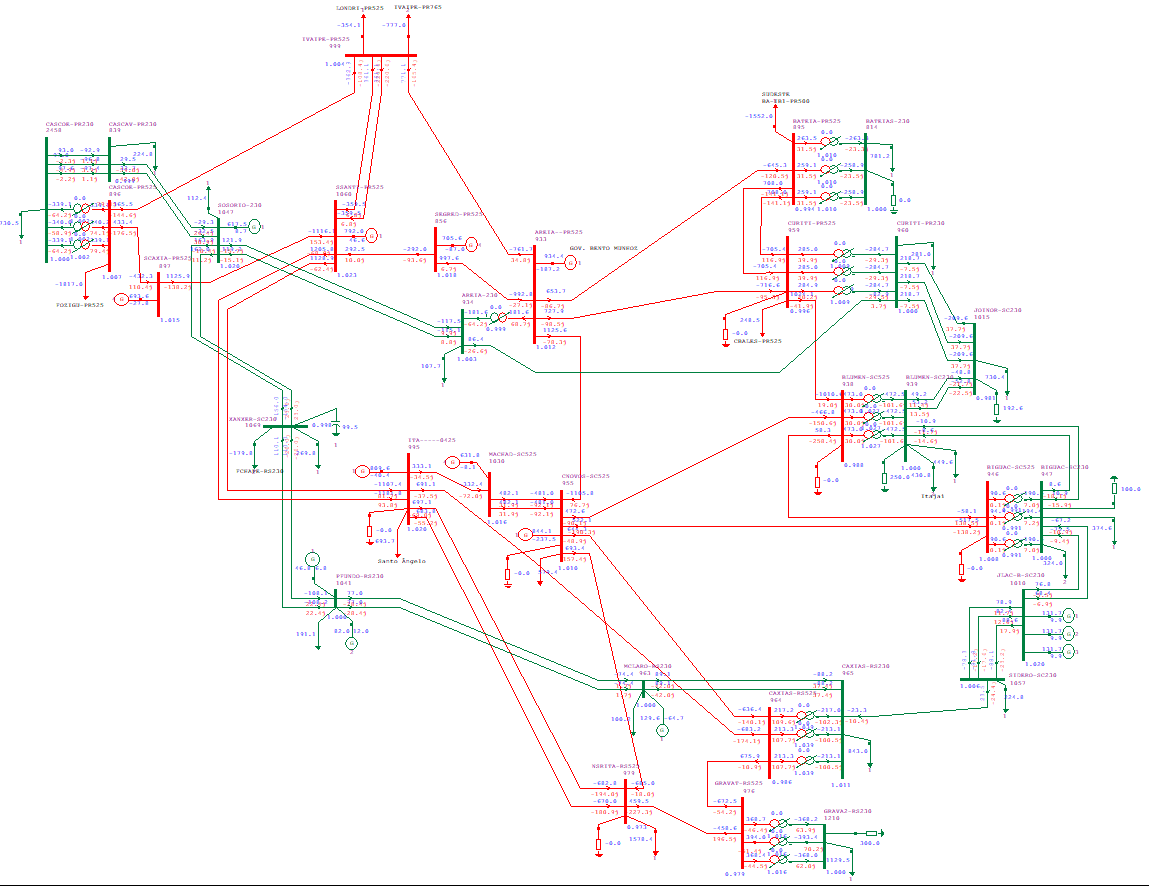
\includegraphics[width=0.5\textwidth]{Figuras/STSB-32.png}
	\centering
	\caption{Diagrama do sistema de transmissão sul brasileiro de 32 barras.}
	\label{figura: Sistema_STSB_32}
\end{figure}

Sendo o sistema separado por tensão, os níveis de tensão são de 230 kV, na cor verde e 525 kV na cor vermelha, esse sistema também é dividido em três áreas. A área número 1 é a parte classificada em 525 kV, a área 2 é a parte do sistema em 230 kV e a área 3 é a área de importação de energia da região sudeste do Brasil.

Para a utilização deste tipo de análise, foi dada a tabela \ref{tabela: Probabilidade_Linhas} com os valores de confiabilidade em cada linha, assim podendo analisar as tabelas de contingências com o diagrama de cortes mínimos.

\begin{table}[!ht]
	\caption{Probabilidade das Linhas STSB-32}
	\label{tabela: Probabilidade_Linhas}
%	\scalefont{0.8}
	\centering
	\begin{tabularx}{.5\textwidth}{|Y|Y|Y|Y|}
		\hline
		De & Para & \textbf{Q} & \textbf{P} \\ \hline
		933 & 856 & 2,79E-04 & 9,9972E-01 \\ \hline
		933 & 895 & 1,26E-03 & 9,9874E-01 \\ \hline
		933 & 955 & 8,66E-04 & 9,9913E-01 \\ \hline
		933 & 959 & 1,16E-03 & 9,9884E-01 \\ \hline
		933 & 999 & 8,51E-04 & 9,9915E-01 \\ \hline
		895 & 959 & 1,65E-04 & 9,9984E-01 \\ \hline
		946 & 938 & 4,28E-04 & 9,9957E-01 \\ \hline
		946 & 955 & 1,15E-03 & 9,9885E-01 \\ \hline
		938 & 955 & 1,24E-03 & 9,9876E-01 \\ \hline
		938 & 959 & 6,78E-04 & 9,9932E-01 \\ \hline
		896 & 897 & 3,10E-04 & 9,9969E-01 \\ \hline
		896 & 999 & 1,03E-03 & 9,9897E-01 \\ \hline
		964 & 955 & 9,99E-04 & 9,9900E-01 \\ \hline
		964 & 976 & 3,87E-04 & 9,9961E-01 \\ \hline
		964 & 995 & 1,25E-03 & 9,9875E-01 \\ \hline
		955 & 979 & 1,26E-03 & 9,9874E-01 \\ \hline
		955 & 1030 & 1,96E-04 & 9,9980E-01 \\ \hline
		976 & 979 & 1,45E-04 & 9,9985E-01 \\ \hline
		995 & 979 & 1,54E-03 & 9,9846E-01 \\ \hline
		995 & 1030 & 3,18E-04 & 9,9968E-01 \\ \hline
		995 & 1060 & 9,19E-04 & 9,9908E-01 \\ \hline
		999 & 1060 & 8,21E-04 & 9,9918E-01 \\ \hline
		897 & 1060 & 4,43E-04 & 9,9956E-01 \\ \hline
		856 & 1060 & 2,98E-04 & 9,9970E-01 \\ \hline
		934 & 960 & 6,59E-04 & 9,9934E-01 \\ \hline
		934 & 1047 & 4,30E-04 & 9,9957E-01 \\ \hline
		947 & 939 & 3,36E-04 & 9,9966E-01 \\ \hline
		947 & 1010 & 3,47E-04 & 9,9965E-01 \\ \hline
		939 & 1015 & 1,96E-04 & 9,9980E-01 \\ \hline
		839 & 1047 & 2,15E-04 & 9,9978E-01 \\ \hline
		839 & 2458 & 2,76E-05 & 9,9997E-01 \\ \hline
		965 & 963 & 1,43E-04 & 9,9986E-01 \\ \hline
		965 & 1057 & 5,64E-04 & 9,9944E-01 \\ \hline
		960 & 1015 & 2,68E-04 & 9,9973E-01 \\ \hline
		1010 & 1057 & 1,27E-04 & 9,9987E-01 \\ \hline
		963 & 1041 & 6,12E-04 & 9,9939E-01 \\ \hline
		1041 & 1069 & 2,12E-04 & 9,9979E-01 \\ \hline
		1047 & 1069 & 4,34E-04 & 9,9957E-01 \\ \hline
	\end{tabularx}
\end{table}

Utilizando a tabela \ref{tabela: Nivel_Carregamento} e \ref{tabela: Nivel_Geracao} para calcular os valores de cada uma das possibilidades para contingências de N-1 e N-2, utilizando os casos de abertura de cada uma das linhas uma única vez, caso alerta de violações do \emph{ANAREDE} seria gerado um relatório e buscado essas informação de qual o valor de \textbf{Q} e \textbf{P} para cada linha.


\section{Resultados}

A utilização da confiabilidade e com uma lista de contingências da primeira ordem qual ele retornou o relatório de violação N-1 da tabela \ref{tabela: N_1}.

\begin{table}[!ht]
	\caption{Relatório de Violação N-1 ANAREDE.}
	\label{tabela: N_1}
	\scalefont{0.7}
	\centering
	\begin{tabularx}{.5\textwidth}{|Y|Y|Y|Y|Y|Y|Y|}
		\hline
		Violação & Cont. & De & Para & Sev. & Q & P \\ \hline
		Tensão & 5 & 896 & 897 & 8,5 & 3,098E-04 & 9,997E-01 \\ \hline
		Tensão & 13 & 938 & 959 & 4,4 & 6,784E-04 & 9,993E-01 \\ \hline
		Tensão & 24 & 995 & 979 & 3 & 1,542E-03 & 9,985E-01 \\ \hline
		Tensão & 20 & 964 & 976 & 1,4 & 3,875E-04 & 9,996E-01 \\ \hline
		Tensão & 23 & 995 & 964 & 1,1 & 1,253E-03 & 9,987E-01 \\ \hline
		Divergente & 17 & 955 & 979 &  & 1,265E-03 & 9,987E-01 \\ \hline
	\end{tabularx}
\end{table}

Assim para o caso N-1, temos a tabela \ref{tabela: N_1} qual apresenta a contingência, de qual barra para qual barra, apresenta o Q e P para cada contingência gerada assim pelo \emph{ANAREDE}. Assim tirando os valores das contingências N-1 para criar uma lista de contingências de N-2, qual será feita os diagramas de cortes mínimos.


\begin{table}[!ht]
	\caption{Relatório de Violação N-2 ANAREDE.}
	\label{tabela: N_2}
	\scalefont{0.7}
	\centering
	\begin{tabularx}{.5\textwidth}{|Y|Y|Y|Y|Y|Y|Y|Y|Y|}
		\hline
		Violação & Cont & De1 & Para1 & Sev & Q1 & De2 & Para2 & Q2 \\ \hline
		Tensão & 509 & 955 & 946 & 9,6 & 1,15E-03 & 960 & 1015 & 1,15E-03 \\ \hline
		Tensão & 517 & 955 & 946 & 5,5 & 1,15E-03 & 1010 & 947 & 1,15E-03 \\ \hline
		Tensão & 508 & 955 & 946 & 5,2 & 1,15E-03 & 959 & 895 & 1,15E-03 \\ \hline
		Tensão & 352 & 933 & 955 & 4,1 & 8,66E-04 & 955 & 946 & 8,66E-04 \\ \hline
		Tensão & 349 & 933 & 955 & 3,5 & 8,66E-04 & 938 & 946 & 8,66E-04 \\ \hline
		Tensão & 487 & 947 & 939 & 3,2 & 3,36E-04 & 955 & 946 & 3,36E-04 \\ \hline
		Tensão & 528 & 955 & 964 & 3,2 & 9,99E-04 & 965 & 1057 & 9,99E-04 \\ \hline
		Tensão & 449 & 938 & 946 & 2,6 & 4,27E-04 & 960 & 1015 & 4,27E-04 \\ \hline
		Tensão & 470 & 938 & 955 & 2,5 & 1,24E-03 & 960 & 1015 & 1,24E-03 \\ \hline
		Tensão & 538 & 955 & 964 & 2,4 & 9,99E-04 & 1047 & 1069 & 9,99E-04 \\ \hline
		Tensão & 507 & 955 & 946 & 2,2 & 1,15E-03 & 955 & 964 & 1,15E-03 \\ \hline
		Tensão & 297 & 856 & 1060 & 1,8 & 2,97E-04 & 938 & 955 & 2,97E-04 \\ \hline
		Tensão & 476 & 938 & 955 & 1,7 & 1,24E-03 & 999 & 933 & 1,24E-03 \\ \hline
		Tensão & 269 & 856 & 933 & 1,2 & 2,78E-04 & 938 & 955 & 2,78E-04 \\ \hline
		Tensão & 448 & 938 & 946 & 1,2 & 4,27E-04 & 959 & 895 & 4,27E-04 \\ \hline
		Tensão & 542 & 955 & 964 & 1,1 & 9,99E-04 & 1041 & 963 & 9,99E-04 \\ \hline
		Tensão & 539 & 955 & 964 & 1,1 & 9,99E-04 & 1057 & 1010 & 9,99E-04 \\ \hline
		Tensão & 272 & 856 & 933 & 1,1 & 2,78E-04 & 955 & 964 & 2,78E-04 \\ \hline
		Tensão & 541 & 955 & 964 & 1,1 & 9,99E-04 & 1069 & 1041 & 9,99E-04 \\ \hline
		Tensão & 353 & 933 & 955 & 1 & 8,66E-04 & 955 & 964 & 8,66E-04 \\ \hline
		Tensão & 468 & 938 & 955 & 1 & 1,24E-03 & 955 & 964 & 1,24E-03 \\ \hline
		Divergentes & 638 & 999 & 896 & ; & 1,02E-03 & 1060 & 897 & 1,02E-03 \\ \hline
		Divergentes & 529 & 955 & 964 & ; & 9,99E-04 & 976 & 979 & 9,99E-04 \\ \hline
		Divergentes & 467 & 938 & 955 & ; & 1,24E-03 & 955 & 946 & 1,24E-03 \\ \hline
		Divergentes & 446 & 938 & 946 & ; & 4,27E-04 & 955 & 946 & 4,27E-04 \\ \hline
		Divergentes & 444 & 938 & 946 & ; & 4,27E-04 & 938 & 955 & 4,27E-04 \\ \hline
		Divergentes & 377 & 933 & 959 & ; & 1,15E-03 & 955 & 946 & 1,15E-03 \\ \hline
		Divergentes & 375 & 933 & 959 & ; & 1,15E-03 & 938 & 955 & 1,15E-03 \\ \hline
		Divergentes & 326 & 933 & 895 & ; & 1,25E-03 & 955 & 946 & 1,25E-03 \\ \hline
		Divergentes & 324 & 933 & 895 & ; & 1,25E-03 & 933 & 959 & 1,25E-03 \\ \hline
		Divergentes & 320 & 933 & 895 & ; & 1,25E-03 & 933 & 959 & 1,25E-03 \\ \hline
	\end{tabularx}
\end{table}

Com a tabela \ref{tabela: N_2} pode-se iniciar o diagrama de cortes mínimos, utilizando os valores de tabelas de Q e P equivalentes, sabendo que (\ref{equacao: Confiabilidade_Estrutural}) podemos converter Q em P ou vice-versa.

\begin{equation}
	1 = P + Q
	\label{equacao: Confiabilidade_Estrutural}
\end{equation}

Com os valores de Q e P podemos definir que a confiabilidade de sistema é o produto da probabilidade de todos os componentes em série, pela equação (\ref{equacao: Confiabilidade_Estrutural_Serie}).

\begin{equation}
	\sum_{i=1}^{n}(p_{i})
	\label{equacao: Confiabilidade_Estrutural_Serie}
\end{equation}

Logo definir a confiabilidade do sistema é 1 menos o produto da probabilidade de falha de todos os componentes em paralelo, pela equação (\ref{equacao: Confiabilidade_Estrutural_Paralelo}).

\begin{equation}
	1-\sum_{i=1}^{n}(1-p_{i})
	\label{equacao: Confiabilidade_Estrutural_Paralelo}
\end{equation}

Utilizando essas equações temos os equivalentes do relatório de violação N-2 da Tabela \ref{tabela: N_2}, utilizando primeiramente a equação \ref{equacao: Confiabilidade_Estrutural_Paralelo}, após essa análise junta-se o relatório N-1 com o equivalente do N-2 Tabela III.

\begin{table}[!ht]
	\caption{Equivalentes de N-2 ANAREDE.}
	\label{tabela: Equivalente_N_2}
	\centering
	\scalefont{0.7}
	\begin{tabularx}{.5\textwidth}{|Y|Y|Y|Y|Y|Y|Y|}
		\hline
		Cont. & De1 & Para1 & De2 & Para2 & Q Eq & P Eq \\ \hline
		509 & 955 & 946 & 960 & 1015 & 1.33056E-06 & 0.999998669 \\ \hline
		517 & 955 & 946 & 1010 & 947 & 1.33056E-06 & 0.999998669 \\ \hline
		508 & 955 & 946 & 959 & 895 & 1.33056E-06 & 0.999998669 \\ \hline
		352 & 933 & 955 & 955 & 946 & 7.50788E-07 & 0.999999249 \\ \hline
		349 & 933 & 955 & 938 & 946 & 7.50788E-07 & 0.999999249 \\ \hline
		487 & 947 & 939 & 955 & 946 & 1.13071E-07 & 0.999999887 \\ \hline
		528 & 955 & 964 & 965 & 1057 & 9.98101E-07 & 0.999999002 \\ \hline
		449 & 938 & 946 & 960 & 1015 & 1.82996E-07 & 0.999999817 \\ \hline
		470 & 938 & 955 & 960 & 1015 & 1.53884E-06 & 0.999998461 \\ \hline
		538 & 955 & 964 & 1047 & 1069 & 9.98101E-07 & 0.999999002 \\ \hline
		507 & 955 & 946 & 955 & 964 & 1.33056E-06 & 0.999998669 \\ \hline
		297 & 856 & 1060 & 938 & 955 & 8.85122E-08 & 0.999999911 \\ \hline
		476 & 938 & 955 & 999 & 933 & 1.53884E-06 & 0.999998461 \\ \hline
		269 & 856 & 933 & 938 & 955 & 7.77462E-08 & 0.999999922 \\ \hline
		448 & 938 & 946 & 959 & 895 & 1.82996E-07 & 0.999999817 \\ \hline
		542 & 955 & 964 & 1041 & 963 & 9.98101E-07 & 0.999999002 \\ \hline
		539 & 955 & 964 & 1057 & 1010 & 9.98101E-07 & 0.999999002 \\ \hline
		272 & 856 & 933 & 955 & 964 & 7.77462E-08 & 0.999999922 \\ \hline
		541 & 955 & 964 & 1069 & 1041 & 9.98101E-07 & 0.999999002 \\ \hline
		353 & 933 & 955 & 955 & 964 & 7.50788E-07 & 0.999999249 \\ \hline
		468 & 938 & 955 & 955 & 964 & 1.53884E-06 & 0.999998461 \\ \hline
		638 & 999 & 896 & 1060 & 897 & 1.05473E-06 & 0.999998945 \\ \hline
		529 & 955 & 964 & 976 & 979 & 9.98101E-07 & 0.999999002 \\ \hline
		467 & 938 & 955 & 955 & 946 & 1.53884E-06 & 0.999998461 \\ \hline
		446 & 938 & 946 & 955 & 946 & 1.82996E-07 & 0.999999817 \\ \hline
		444 & 938 & 946 & 938 & 955 & 1.82996E-07 & 0.999999817 \\ \hline
		377 & 933 & 959 & 955 & 946 & 1.33541E-06 & 0.999998665 \\ \hline
		375 & 933 & 959 & 938 & 955 & 1.33541E-06 & 0.999998665 \\ \hline
		326 & 933 & 895 & 955 & 946 & 1.58181E-06 & 0.999998418 \\ \hline
		324 & 933 & 895 & 933 & 959 & 1.58181E-06 & 0.999998418 \\ \hline
		320 & 933 & 895 & 933 & 959 & 1.58181E-06 & 0.999998418 \\ \hline
	\end{tabularx}
\end{table}

Assim com o equivalente de cada uma das linhas de transmissão feitos vamos calcular o múltiplo como se todos os elementos fossem série juntamente com a lista contingências N-1 da Tabela \ref{tabela: N_1}, pode-se calcular a Tabela \ref{tabela: Equivalente_Sistema}, qual representa o resultado da confiabilidade.

\begin{table}[!ht]
	\caption{Resultantes de Confiabilidade do sistema.}
	\label{tabela: Equivalente_Sistema}
	\centering
	\scalefont{0.6}
	\begin{tabularx}{.5\textwidth}{|Y|Y|Y|Y|Y|Y|Y|}
		\hline
			Cont & De1 & Para1 & De2 & Para2 & Q & P \\ \hline
			5 & 896 & 897 & - & - & 3.098100E-04 & 9.996902E-01 \\ \hline
			13 & 938 & 959 & - & - & 6.783700E-04 & 9.993216E-01 \\ \hline
			17 & 955 & 979 & - & - & 1.264600E-03 & 9.987354E-01 \\ \hline
			20 & 964 & 976 & - & - & 3.874700E-04 & 9.996125E-01 \\ \hline
			23 & 995 & 964 & - & - & 1.252800E-03 & 9.987472E-01 \\ \hline
			24 & 995 & 979 & - & - & 1.542200E-03 & 9.984578E-01 \\ \hline
			269 & 856 & 933 & 938 & 955 & 7.774617E-08 & 9.999999E-01 \\ \hline
			272 & 856 & 933 & 955 & 964 & 7.774617E-08 & 9.999999E-01 \\ \hline
			297 & 856 & 1060 & 938 & 955 & 8.851220E-08 & 9.999999E-01 \\ \hline
			320 & 933 & 895 & 933 & 959 & 1.581809E-06 & 9.999984E-01 \\ \hline
			324 & 933 & 895 & 933 & 959 & 1.581809E-06 & 9.999984E-01 \\ \hline
			326 & 933 & 895 & 955 & 946 & 1.581809E-06 & 9.999984E-01 \\ \hline
			349 & 933 & 955 & 938 & 946 & 7.507876E-07 & 9.999992E-01 \\ \hline
			352 & 933 & 955 & 955 & 946 & 7.507876E-07 & 9.999992E-01 \\ \hline
			353 & 933 & 955 & 955 & 964 & 7.507876E-07 & 9.999992E-01 \\ \hline
			375 & 933 & 959 & 938 & 955 & 1.335411E-06 & 9.999987E-01 \\ \hline
			377 & 933 & 959 & 955 & 946 & 1.335411E-06 & 9.999987E-01 \\ \hline
			444 & 938 & 946 & 938 & 955 & 1.829957E-07 & 9.999998E-01 \\ \hline
			446 & 938 & 946 & 955 & 946 & 1.829957E-07 & 9.999998E-01 \\ \hline
			448 & 938 & 946 & 959 & 895 & 1.829957E-07 & 9.999998E-01 \\ \hline
			449 & 938 & 946 & 960 & 1015 & 1.829957E-07 & 9.999998E-01 \\ \hline
			467 & 938 & 955 & 955 & 946 & 1.538840E-06 & 9.999985E-01 \\ \hline
			468 & 938 & 955 & 955 & 964 & 1.538840E-06 & 9.999985E-01 \\ \hline
			470 & 938 & 955 & 960 & 1015 & 1.538840E-06 & 9.999985E-01 \\ \hline
			476 & 938 & 955 & 999 & 933 & 1.538840E-06 & 9.999985E-01 \\ \hline
			487 & 947 & 939 & 955 & 946 & 1.130708E-07 & 9.999999E-01 \\ \hline
			507 & 955 & 946 & 955 & 964 & 1.330562E-06 & 9.999987E-01 \\ \hline
			508 & 955 & 946 & 959 & 895 & 1.330562E-06 & 9.999987E-01 \\ \hline
			509 & 955 & 946 & 960 & 1015 & 1.330562E-06 & 9.999987E-01 \\ \hline
			517 & 955 & 946 & 1010 & 947 & 1.330562E-06 & 9.999987E-01 \\ \hline
			528 & 955 & 964 & 965 & 1057 & 9.981009E-07 & 9.999990E-01 \\ \hline
			529 & 955 & 964 & 976 & 979 & 9.981009E-07 & 9.999990E-01 \\ \hline
			538 & 955 & 964 & 1047 & 1069 & 9.981009E-07 & 9.999990E-01 \\ \hline
			539 & 955 & 964 & 1057 & 1010 & 9.981009E-07 & 9.999990E-01 \\ \hline
			541 & 955 & 964 & 1069 & 1041 & 9.981009E-07 & 9.999990E-01 \\ \hline
			542 & 955 & 964 & 1041 & 963 & 9.981009E-07 & 9.999990E-01 \\ \hline
			638 & 999 & 896 & 1060 & 897 & 1.054729E-06 & 9.999989E-01 \\ \hline
			Total & ~ & ~ & ~ & ~ & 5.45274E-03 & 9.94547E-01 \\ \hline
			Total (\%) & ~ & ~ & ~ & ~ & 0.005452738 & 0.994547262 \\ \hline
	\end{tabularx}
\end{table}

\newpage

Assim com as contingências apresentadas em N-1 Tabela \ref{tabela: N_1} e N-2 Tabela \ref{tabela: Equivalente_N_2}, temos os valores de falha em cada uma das linhas separados assim aplicando as formulas de confiabilidade podemos determinar o resultante total da tabela \ref{tabela: Equivalente_Sistema}. Assim determinamos os resultados na tabela \ref{tabela: Resultado_Confiabilidade}.

\begin{table}[!ht]
	\caption{Resultado da Análise de Confiabilidade do Sistema STSB-32.}
	\label{tabela: Resultado_Confiabilidade}
	\centering
%	\scalefont{0.5}
	\begin{tabularx}{.5\textwidth}{|Y|Y|Y|Y|}
		\hline
		Total & 5.45274E-03 & 9.94547E-01 & 1.00000E+00 \\ \hline
		Total (\%) & 0.005452738 & 0.994547262 & 1 \\ \hline
	\end{tabularx}
\end{table}


\section{Conclusão}
The conclusion goes here.


%{\appendices
%\section*{Proof of the First Zonklar Equation}
%Appendix one text goes here.
% You can choose not to have a title for an appendix if you want by leaving the argument blank
%\section*{Proof of the Second Zonklar Equation}
%Appendix two text goes here.}
 
\bibliography{LeonardoReferencias}
\bibliographystyle{IEEEtran}

\end{document}



